\section{Introduction}\label{sec:intro}

Over an imperfect field, a regular variety need not be smooth, and its base change to an algebraic closure need not be normal or even reduced.
Let $k$ be a field of characteristic $p>0$, and let $X$ be a regular projective surface over $k$ with $H^0(X,\O_X) = k$ and $K_X \equiv 0$.
Wang and Zhang proved that such a surface is geometrically integral if $p\geq 7$ \cite[Theorem~1.2]{WZ26}.
If moreover $p\geq 7$ and $X$ is not geometrically normal, then every numerically trivial line bundle on $X$ is trivial, in particular $K_X\sim 0$ \cite[Corollary~6.2]{CWZ26}.
Wang and Zhang also exhibit, for $p = 5$ and $p = 7$, examples with $K_X \equiv 0$ which are geometrically integral but not geometrically normal, and they ask whether geometric normality holds in large characteristic \cite[Question~1.1 and Remark~1.5(2)]{WZ26}.
We prove that it does for $p\geq 13$.

\begin{theorem}[{Theorem~\ref{thm:geometric-normality}}]\label{thm:main}
Let $k$ be a field of characteristic $p\geq 13$, and let $X$ be a regular projective surface over $k$ with $H^0(X,\O_X) = k$ and $K_X\equiv 0$.
Then $X$ is geometrically normal over $k$.
\end{theorem}

The bound $p\geq 13$ is optimal.

\begin{theorem}[{Proposition~\ref{prop:p11}}]\label{thm:intro-p11}
Let $k$ be the field $\FF_{11}(c)$, with $c$ transcendental over $\FF_{11}$.
Then there is a regular projective surface $X$ over $k$ with $H^0(X,\O_X) = k$ and $\omega_X\cong\O_X$ which is not geometrically normal over $k$.
\end{theorem}

The surface $X$ is fibred over $\PP^1_k$, with coordinate $u$, in curves of genus one.
Its generic fibre is a twist, by an $\alpha_{11}$-torsor, of the elliptic curve $y^2 = x^3+u^5$.
The fibre over $u = 0$ is an integral curve, but $X_{k(c^{1/11})}$ is not normal along it.
Over this point the Jacobian has reduction of type $\mathrm{II}^*$, which is precisely the configuration that the argument of Section~\ref{sec:genus-one} leaves open for $p = 11$ (Remark~\ref{rem:small-primes}).

\smallskip
For $p\geq 23$, we obtain the stronger conclusion of smoothness.

\begin{theorem}[{Theorem~\ref{thm:smooth}}]\label{thm:intro-smooth}
Let $k$ be a field of characteristic $p\geq 23$, and let $X$ be a regular projective surface over $k$ with $H^0(X,\O_X) = k$ and $K_X\equiv 0$.
Then $X$ is smooth over $k$.
\end{theorem}

The bound $p\geq 23$ is optimal.
\begin{theorem}[{Proposition~\ref{prop:small-primes-sing} and Example~\ref{ex:small-primes}}]\label{thm:intro-small-primes}
Let $k$ be a field of characteristic $p\in\{13,17,19\}$, and let $X$ be a regular projective surface over $k$ with $H^0(X,\O_X) = k$ and $K_X\equiv 0$.
Then $X_{\bar k}$ is either smooth or has exactly one singular point, of type $\mathrm A_{p-1}$.
For each such $p$, the singular case occurs over $k = \FF_p(c)$, with $c$ transcendental over $\FF_p$.
\end{theorem}

\begin{remark}\label{rem:intro-smooth-optimal}
For $p = 19$, the example in Theorem~\ref{thm:intro-small-primes} is the special fibre of a regular flat projective model over $\ZZ[c]_{(19)}$ with K3 generic fibre and trivial relative canonical sheaf (Proposition~\ref{prop:small-primes-lift}).
This model shows that the bound $p\geq 23$ in Corollary~\ref{cor:mixed-smooth} is optimal in mixed characteristic, even when both the total space and the special fibre are regular.
\end{remark}

For completeness, we show that regular surfaces with nef anticanonical class and $K_X\not\equiv 0$ are geometrically normal for $p\geq 5$ and smooth for $p\geq 11$.
\begin{theorem}[{Proposition~\ref{prop:nef-nontrivial}}]\label{thm:intro-nef}
Let $k$ be a field of characteristic $p\geq 5$, and let $X$ be a regular projective surface over $k$ with $H^0(X,\O_X) = k$ such that $-K_X$ is nef and $K_X\not\equiv 0$.
Then $X$ is geometrically normal over $k$, and $X_{\bar k}$ has at worst rational double points.
If moreover $p\geq 11$, then $X$ is smooth over $k$.
\end{theorem}

Both bounds in Theorem~\ref{thm:intro-nef} are optimal, already for del Pezzo surfaces.
In characteristics $2$ and $3$ there are regular del Pezzo surfaces which are not geometrically normal \cite[Example~2.3]{Ber24}.
In characteristic $7$ there is a regular del Pezzo surface of degree $2$ whose geometric base change has a singular point of type $\mathrm A_6$, so it is not smooth \cite[Example~2.3]{MS24}.

The genus-one argument uses a local result for minimal regular models over excellent discrete valuation rings of equal characteristic $p>0$.
If the Jacobian has good reduction and the closed fibre is reduced, then the discrepancy $b$ between the lattices of relative differentials is either zero, in which case the model is smooth, or at least $p-1$ (Corollary~\ref{lem:congruence}).
For the surfaces considered here, a tame base change gives $b\leq 11$, so this local result supplies the contradiction for $p\geq 13$ in the potentially good reduction case.

\subsection{Proof strategy of Theorem~\ref{thm:main}}

Suppose that $p\geq 13$ and that $X$ is not geometrically normal.
We may assume that $k$ is $F$-finite and separably closed.
The main step in the genus-one case compares the relative dualizing sheaves of the fibration and its Jacobian after tame base change.
In the anisotropic case, we contract a negative curve while preserving failure of geometric normality, then exclude the resulting surface of Picard number one.
Figure~\ref{fig:strategy-main} shows the structure of the argument.

\begin{figure}[ht]
\centering
\begin{tikzpicture}[
  box/.style={draw, rounded corners, align=flush center, font=\small, inner sep=4pt},
  last/.style={box, fill=gray!12},
  lab/.style={font=\footnotesize, fill=white, inner sep=1pt},
]
\node[box, text width=11cm] (s) at (0,0) {Assume $p\geq 13$, and $X$ is not geometrically normal};
\node[box, text width=11cm, anchor=north] (a) at ([yshift=-5mm]s.south) {$\omega_X\cong\O_X$, $H^1(X,\O_X) = 0$ and $\chi(\O_X) = 2$ \quad(Section~\ref{sec:torsors})};
\node[box, text width=11cm, anchor=north] (b) at ([yshift=-5mm]a.south) {$\Pic(X)$ is an even lattice with $\lvert\det\rvert = p^a$ \quad(Section~\ref{sec:torsors})};
\node[box, text width=7.4cm, anchor=north] (c) at ([xshift=-4.2cm,yshift=-13mm]b.south) {Genus-one fibration $f\from X\to\PP^1$, with $J$ the Jacobian of its generic fibre \quad(Section~\ref{sec:genus-one})};
\node[box, text width=6.2cm, anchor=north] (d) at ([xshift=4.4cm,yshift=-13mm]b.south) {$\rho(X) = 2$; contracting a negative curve gives $X\to X'$ with $\rho(X') = 1$ and $X'$ not geometrically normal \quad(Section~\ref{sec:rank-two})};
\node[box, text width=3.45cm, anchor=north] (c1) at ([xshift=-1.95cm,yshift=-5mm]c.south) {Good or multiplicative reduction: normal by reduction theory};
\node[box, text width=3.45cm, anchor=north] (c2) at ([xshift=1.95cm,yshift=-5mm]c.south) {Additive reduction: after a tame base change, $J$ has good reduction ($b = 0$, as $(p-1)\mid b\leq 11$) or multiplicative reduction (different exponent $\leq 3<p-1$)};
\node[last, text width=7.4cm, anchor=north] (ce) at ([xshift=-1.95cm,yshift=-5mm]c2.south) {$X_{\bar k}$ is normal along every fibre of $f$: contradiction \quad(Proposition~\ref{prop:genus-one})};
\node[last, text width=6.2cm, anchor=north] (e) at ([yshift=-5mm]d.south) {The normalization $S'$ of $X'_{\bar k}$ is rational with $-K_{S'}\sim(p-1)D'$ for a nonzero effective $\ZZ$-divisor $D'$. The resolution configurations give $(-K_{S'})\cdot A\notin(p-1)\ZZ_{>0}$ for a suitable ample Cartier divisor $A$ on $S'$, a contradiction \quad(Section~\ref{sec:rank-one})};
\draw[->] (s) -- (a);
\draw[->] (a) -- (b);
\draw[->] (b.south) -- ++(0,-6.5mm) -| node[lab, pos=0.25] {isotropic class} (c.north);
\draw[->] (b.south) -- ++(0,-6.5mm) -| node[lab, pos=0.25] {no isotropic class} (d.north);
\draw[->] (c.south) -- ++(0,-2.5mm) -| (c1.north);
\draw[->] (c.south) -- ++(0,-2.5mm) -| (c2.north);
\draw[->] (c1.south) -- (c1.south |- ce.north);
\draw[->] (c2.south) -- (c2.south |- ce.north);
\draw[->] (d) -- (e);
\end{tikzpicture}
\caption{Structure of the proof of Theorem~\ref{thm:main}.}
\label{fig:strategy-main}
\end{figure}

\subsection{Proof strategy of Theorem~\ref{thm:intro-smooth}}

Assume now that $p\geq 23$.
By Theorem~\ref{thm:main}, the geometric surface $Y := X_{\bar k}$ is normal.
We may assume that $k$ is $F$-finite and separably closed.
The elliptic case is excluded by combining a local bound $d\leq 3$ on the degree of the singularity with a computer-assisted enumeration forcing $d = 4$.
The computation is needed only when $p\equiv 1\pmod 4$ and $p\leq 6912$.
Figure~\ref{fig:strategy-smooth} shows the structure of the argument.

\begin{figure}[ht]
\centering
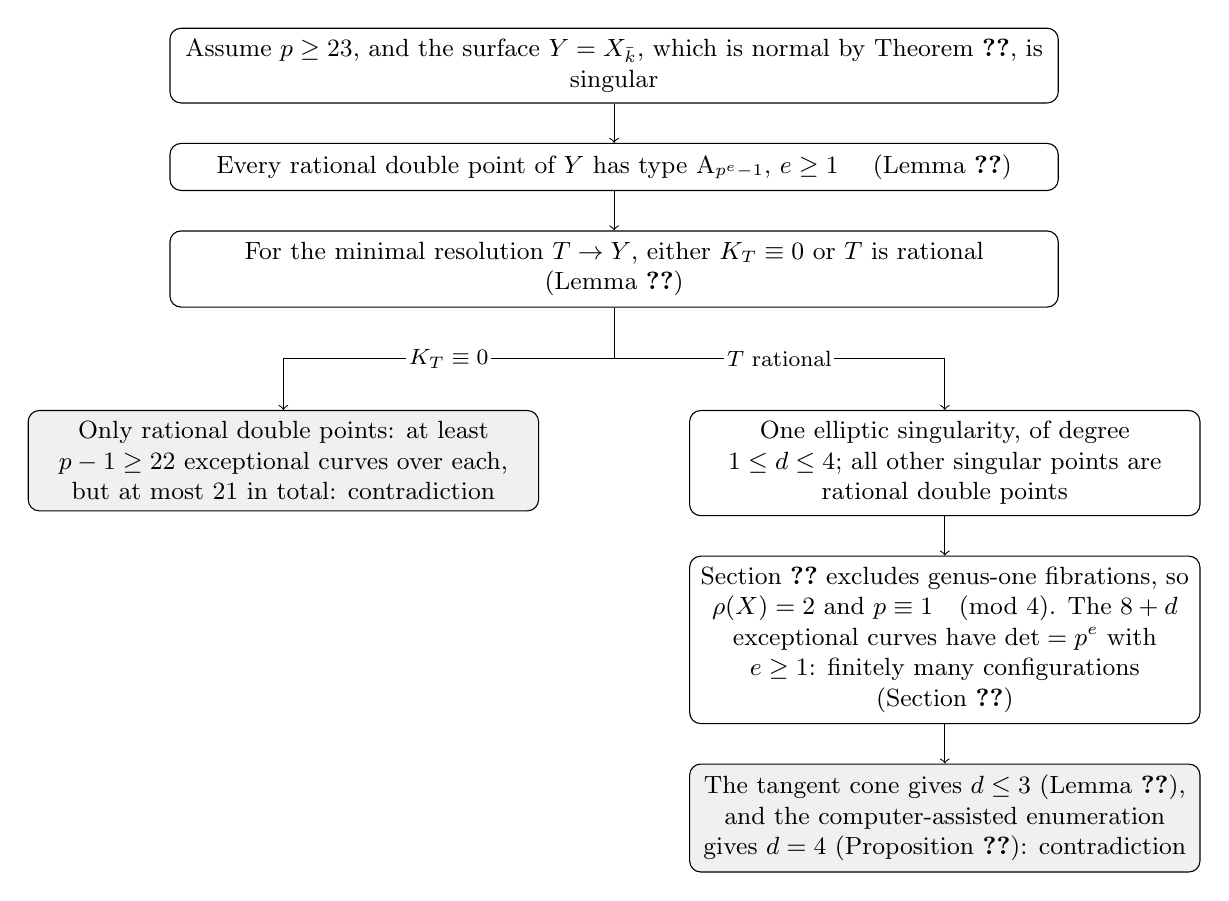
\begin{tikzpicture}[
  box/.style={draw, rounded corners, align=flush center, font=\small, inner sep=4pt},
  last/.style={box, fill=gray!12},
  lab/.style={font=\footnotesize, fill=white, inner sep=1pt},
]
\node[box, text width=11cm] (s) at (0,0) {Assume $p\geq 23$, and the surface $Y = X_{\bar k}$, which is normal by Theorem~\ref{thm:main}, is singular};
\node[box, text width=11cm, anchor=north] (a) at ([yshift=-5mm]s.south) {Every rational double point of $Y$ has type $\mathrm A_{p^e-1}$, $e\geq 1$ \quad(Lemma~\ref{lem:geometric-rdp})};
\node[box, text width=11cm, anchor=north] (b) at ([yshift=-5mm]a.south) {For the minimal resolution $T\to Y$, either $K_T\equiv 0$ or $T$ is rational \quad(Lemma~\ref{lem:smooth-structure})};
\node[last, text width=6.2cm, anchor=north] (l) at ([xshift=-4.2cm,yshift=-13mm]b.south) {Only rational double points: at least $p-1\geq 22$ exceptional curves over each, but at most $21$ in total: contradiction};
\node[box, text width=6.2cm, anchor=north] (r) at ([xshift=4.2cm,yshift=-13mm]b.south) {One elliptic singularity, of degree $1\leq d\leq 4$; all other singular points are rational double points};
\node[box, text width=6.2cm, anchor=north] (c) at ([yshift=-5mm]r.south) {Section~\ref{sec:genus-one} excludes genus-one fibrations, so $\rho(X) = 2$ and $p\equiv 1\pmod 4$. The $8+d$ exceptional curves have $\lvert\det\rvert = p^e$ with $e\geq 1$: finitely many configurations \quad(Section~\ref{sec:smooth})};
\node[last, text width=6.2cm, anchor=north] (d) at ([yshift=-5mm]c.south) {The tangent cone gives $d\leq 3$ (Lemma~\ref{lem:smooth-tangent}), and the computer-assisted enumeration gives $d = 4$ (Proposition~\ref{prop:smooth-enum}): contradiction};
\draw[->] (s) -- (a);
\draw[->] (a) -- (b);
\draw[->] (b.south) -- ++(0,-6.5mm) -| node[lab, pos=0.25] {$K_T\equiv 0$} (l.north);
\draw[->] (b.south) -- ++(0,-6.5mm) -| node[lab, pos=0.25] {$T$ rational} (r.north);
\draw[->] (r) -- (c);
\draw[->] (c) -- (d);
\end{tikzpicture}
\caption{Structure of the proof of Theorem~\ref{thm:intro-smooth}.}
\label{fig:strategy-smooth}
\end{figure}

\subsection*{Acknowledgements}
The author thanks Lei Zhang for sharing an initial draft of this work, which was generated by Jie Liu using ChatGPT.
That draft showed that the surfaces studied here are smooth for $p\geq p_0$, with an ineffective constant $p_0$.
The author improved this result with the help of Claude Code, and contributed mainly by reorganizing the exposition.
